\documentclass[margin=5mm]{standalone}
\usepackage[dvipsnames]{xcolor}
\usepackage{pgfplots}
\usepackage{tikz}
\usepackage[tikz]{ocgx2}

\pgfplotsset{compat=1.18}
\begin{document}

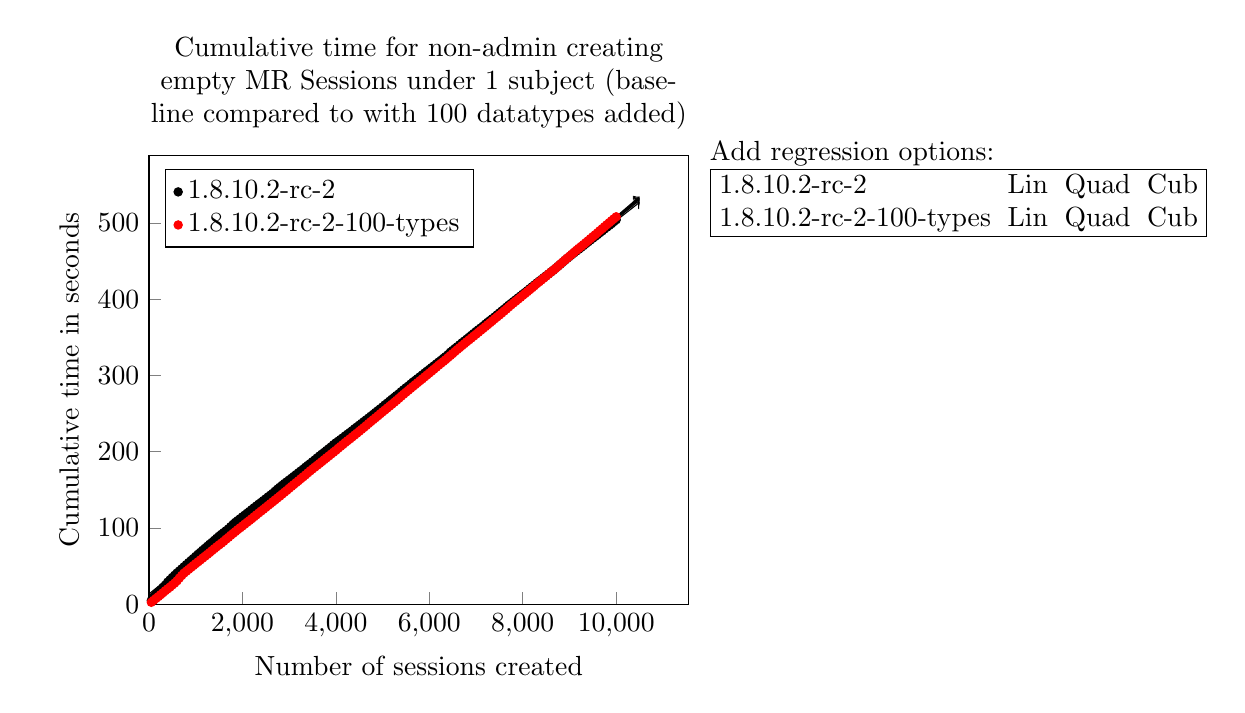
\begin{tikzpicture}
    \begin{axis}[
        align = center,
        legend pos = north west,
        legend cell align = left,
        xlabel = Number of sessions created,
        ylabel = Cumulative time in seconds,
        xtick pos = left,
        ytick pos = left,
        scaled ticks = false,
        xmin = 0,
        ymin = 0,
        title = {Cumulative time for non-admin creating empty MR Sessions under 1 subject  (baseline compared to with 100 datatypes added)},
        title style = {text width = 0.8\textwidth},
        legend entries={\switchocg{1.8.10.2-rc-2}{1.8.10.2-rc-2},\switchocg{1.8.10.2-rc-2-100-types}{1.8.10.2-rc-2-100-types}}]
        \begin{scope}[ocg = {ref = 1.8.10.2-rc-2-Lin, status = invisible}]
            \plot[domain=0:10500,->,forget plot] (\x,{13.39806673366848599471268244087696075439453125 + 0.049153354878871964583897380407506716437637805938720703125*(\x)^1});
        \end{scope}
        \begin{scope}[ocg = {ref = 1.8.10.2-rc-2-Quad, status = invisible}]
            \plot[domain=0:10500,->,forget plot] (\x,{11.3607774577434188501001699478365480899810791015625 + 0.050363625735857141252349578053326695226132869720458984375*(\x)^1 + -0.000000120424960894047387097510683380552354293513417360372841358184814453125*(\x)^2});
        \end{scope}
        \begin{scope}[ocg = {ref = 1.8.10.2-rc-2-Cub, status = invisible}]
            \plot[domain=0:10500,->,forget plot] (\x,{7.97833625410568014757473065401427447795867919921875 + 0.054352705452317580381293993241342832334339618682861328125*(\x)^1 + -0.00000111026289787041589139475472602924810416880063712596893310546875*(\x)^2 + 0.0000000000656608913417159752910936984133540537944551118698655045591294765472412109375*(\x)^3});
        \end{scope}
        \begin{scope}[ocg = {ref = 1.8.10.2-rc-2, status = visible}]
            \addplot[
                only marks,
                color = black,
                mark = *,
                mark size = 1.5 pt
            ]coordinates {(50,4.801)(100,8.607)(150,12.214)(200,15.394)(250,18.591)(300,22.121)(350,25.087)(400,28.912)(450,31.916)(500,35.01)(550,37.945)(600,40.849)(650,43.543)(700,46.21)(750,49.067)(800,51.781)(850,54.547)(900,57.229)(950,59.817)(1000,62.639)(1050,65.406)(1100,67.927)(1150,70.677)(1200,73.279)(1250,75.937)(1300,78.618)(1350,81.059)(1400,83.759)(1450,86.449)(1500,89.119)(1550,91.569)(1600,93.873)(1650,96.233)(1700,98.713)(1750,101.648)(1800,104.62)(1850,107.295)(1900,109.647)(1950,111.988)(2000,114.433)(2050,116.735)(2100,119.217)(2150,121.529)(2200,123.939)(2250,126.408)(2300,128.814)(2350,131.164)(2400,133.467)(2450,135.82)(2500,138.161)(2550,140.645)(2600,142.958)(2650,145.305)(2700,148.142)(2750,150.834)(2800,153.268)(2850,155.813)(2900,158.198)(2950,160.504)(3000,162.798)(3050,165.121)(3100,167.498)(3150,169.899)(3200,172.281)(3250,174.668)(3300,177.009)(3350,179.609)(3400,181.98)(3450,184.26)(3500,186.808)(3550,189.21)(3600,191.773)(3650,194.316)(3700,196.689)(3750,199.024)(3800,201.552)(3850,203.946)(3900,206.369)(3950,209.075)(4000,211.465)(4050,213.698)(4100,215.921)(4150,218.166)(4200,220.62)(4250,222.881)(4300,225.149)(4350,227.504)(4400,230.018)(4450,232.275)(4500,234.676)(4550,237.001)(4600,239.397)(4650,241.725)(4700,244.052)(4750,246.493)(4800,248.936)(4850,251.377)(4900,253.796)(4950,256.192)(5000,258.582)(5050,261.307)(5100,263.652)(5150,266.136)(5200,268.746)(5250,271.178)(5300,273.602)(5350,275.997)(5400,278.71)(5450,281.185)(5500,283.678)(5550,285.993)(5600,288.579)(5650,291.169)(5700,293.481)(5750,295.802)(5800,298.226)(5850,300.631)(5900,303.091)(5950,305.531)(6000,307.865)(6050,310.264)(6100,312.616)(6150,315.096)(6200,317.444)(6250,319.797)(6300,322.352)(6350,324.653)(6400,327.258)(6450,330.397)(6500,332.731)(6550,335.32)(6600,337.626)(6650,340.135)(6700,342.728)(6750,345.092)(6800,347.495)(6850,349.99)(6900,352.496)(6950,354.926)(7000,357.503)(7050,359.829)(7100,362.154)(7150,364.53)(7200,367.188)(7250,369.644)(7300,372.039)(7350,374.351)(7400,376.702)(7450,379.282)(7500,381.865)(7550,384.348)(7600,386.855)(7650,389.474)(7700,392.038)(7750,394.404)(7800,396.837)(7850,399.166)(7900,401.624)(7950,403.995)(8000,406.418)(8050,408.779)(8100,411.213)(8150,413.72)(8200,416.197)(8250,418.624)(8300,421.111)(8350,423.428)(8400,425.795)(8450,428.168)(8500,430.521)(8550,432.941)(8600,435.329)(8650,437.708)(8700,440.237)(8750,442.919)(8800,445.446)(8850,448.062)(8900,450.781)(8950,453.377)(9000,455.819)(9050,458.336)(9100,460.804)(9150,463.162)(9200,465.457)(9250,467.867)(9300,470.192)(9350,472.749)(9400,475.117)(9450,477.524)(9500,479.925)(9550,482.31)(9600,484.599)(9650,487.085)(9700,489.425)(9750,491.961)(9800,494.309)(9850,496.632)(9900,498.956)(9950,501.625)(10000,504.045)};
        \end{scope}
        \begin{scope}[ocg = {ref = 1.8.10.2-rc-2-100-types-Lin, status = invisible}]
            \plot[domain=0:10500,->,forget plot] (\x,{0.5282566834170341341092580478289164602756500244140625 + 0.050544743943598612057055419199969037435948848724365234375*(\x)^1});
        \end{scope}
        \begin{scope}[ocg = {ref = 1.8.10.2-rc-2-100-types-Quad, status = invisible}]
            \plot[domain=0:10500,->,forget plot] (\x,{2.03637392492758362294580365414731204509735107421875 + 0.049648832711018074659303778162211528979241847991943359375*(\x)^1 + 0.0000000891453962766707546491856662372599284793750484823249280452728271484375*(\x)^2});
        \end{scope}
        \begin{scope}[ocg = {ref = 1.8.10.2-rc-2-100-types-Cub, status = invisible}]
            \plot[domain=0:10500,->,forget plot] (\x,{1.2216740727015686918122128190589137375354766845703125 + 0.050609648423652807414097054561352706514298915863037109375*(\x)^1 + -0.000000149268451128897323246743126211322216789767480804584920406341552734375*(\x)^2 + 0.00000000001581518059075078305584415118003140977853693271981683210469782352447509765625*(\x)^3});
        \end{scope}
        \begin{scope}[ocg = {ref = 1.8.10.2-rc-2-100-types, status = visible}]
            \addplot[
                only marks,
                color = red,
                mark = *,
                mark size = 1.5 pt
            ]coordinates {(50,2.453)(100,4.986)(150,7.509)(200,9.895)(250,12.386)(300,14.971)(350,17.648)(400,20.017)(450,22.444)(500,25.132)(550,27.642)(600,30.568)(650,34.219)(700,37.581)(750,40.721)(800,43.213)(850,45.672)(900,48.173)(950,50.614)(1000,53.09)(1050,55.497)(1100,57.979)(1150,60.422)(1200,62.825)(1250,65.246)(1300,67.689)(1350,70.286)(1400,72.779)(1450,75.233)(1500,77.657)(1550,80.002)(1600,82.408)(1650,85.145)(1700,87.54)(1750,90.285)(1800,92.758)(1850,95.213)(1900,97.717)(1950,100.107)(2000,102.459)(2050,104.92)(2100,107.334)(2150,109.683)(2200,112.069)(2250,114.642)(2300,117.097)(2350,119.573)(2400,122.055)(2450,124.383)(2500,126.851)(2550,129.399)(2600,131.8)(2650,134.235)(2700,136.729)(2750,139.197)(2800,141.646)(2850,144.212)(2900,146.753)(2950,149.127)(3000,151.888)(3050,154.396)(3100,156.841)(3150,159.449)(3200,161.847)(3250,164.465)(3300,166.939)(3350,169.463)(3400,172.168)(3450,174.753)(3500,177.21)(3550,179.653)(3600,182.075)(3650,184.479)(3700,186.899)(3750,189.445)(3800,191.861)(3850,194.321)(3900,196.832)(3950,199.229)(4000,201.602)(4050,204.337)(4100,206.858)(4150,209.301)(4200,211.961)(4250,214.342)(4300,216.682)(4350,219.201)(4400,221.692)(4450,224.161)(4500,226.645)(4550,229.166)(4600,231.642)(4650,234.232)(4700,236.865)(4750,239.429)(4800,241.942)(4850,244.435)(4900,246.945)(4950,249.591)(5000,252.142)(5050,254.585)(5100,257.154)(5150,259.62)(5200,262.133)(5250,264.754)(5300,267.265)(5350,269.918)(5400,272.689)(5450,275.278)(5500,277.83)(5550,280.377)(5600,282.954)(5650,285.441)(5700,287.966)(5750,290.49)(5800,292.97)(5850,295.395)(5900,297.972)(5950,300.525)(6000,303.058)(6050,305.548)(6100,308.125)(6150,310.693)(6200,313.348)(6250,315.802)(6300,318.23)(6350,320.67)(6400,323.381)(6450,326.012)(6500,328.558)(6550,331.324)(6600,333.959)(6650,336.417)(6700,339.031)(6750,341.53)(6800,344.098)(6850,346.517)(6900,349.036)(6950,351.473)(7000,353.929)(7050,356.477)(7100,359.027)(7150,361.451)(7200,363.95)(7250,366.451)(7300,369.045)(7350,371.563)(7400,374.157)(7450,376.656)(7500,379.13)(7550,381.662)(7600,384.33)(7650,386.91)(7700,389.656)(7750,392.326)(7800,394.862)(7850,397.293)(7900,399.817)(7950,402.299)(8000,404.858)(8050,407.33)(8100,409.834)(8150,412.331)(8200,414.881)(8250,417.518)(8300,420.218)(8350,422.665)(8400,425.145)(8450,427.674)(8500,430.162)(8550,432.732)(8600,435.311)(8650,437.756)(8700,440.211)(8750,442.811)(8800,445.687)(8850,448.263)(8900,451.046)(8950,453.686)(9000,456.186)(9050,458.806)(9100,461.476)(9150,464.115)(9200,466.66)(9250,469.122)(9300,471.59)(9350,474.124)(9400,476.673)(9450,479.327)(9500,481.926)(9550,484.402)(9600,487.04)(9650,489.774)(9700,492.339)(9750,495.042)(9800,497.638)(9850,500.225)(9900,502.832)(9950,505.358)(10000,507.958)};
        \end{scope}
    \end{axis}
    \begin{scope}
        \addtolength{\tabcolsep}{-0.3em}
        \node [below right, shape=rectangle, align=left](regressiontable) at (7,6) {
            Add regression options: \\
            \begin{tabular}{|llll|}
                \hline
                1.8.10.2-rc-2 & \switchocg{1.8.10.2-rc-2-Lin}{Lin} & \switchocg{1.8.10.2-rc-2-Quad}{Quad} & \switchocg{1.8.10.2-rc-2-Cub}{Cub} \\
                1.8.10.2-rc-2-100-types & \switchocg{1.8.10.2-rc-2-100-types-Lin}{Lin} & \switchocg{1.8.10.2-rc-2-100-types-Quad}{Quad} & \switchocg{1.8.10.2-rc-2-100-types-Cub}{Cub} \\
                \hline
            \end{tabular}
        };
    \end{scope}
\end{tikzpicture}

\end{document}